\documentclass[tikz]{standalone}
\usetikzlibrary{arrows.meta,positioning}

\begin{document}
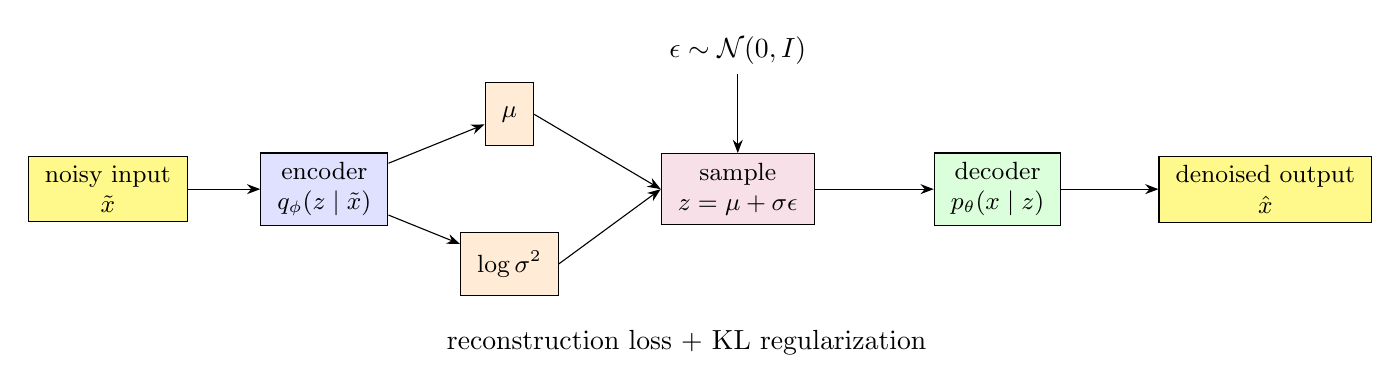
\begin{tikzpicture}[
  >=Stealth,
  block/.style={draw,align=center,minimum height=8mm,inner xsep=6pt,font=\small},
]
  \node[block,fill=yellow!45] (x) at (0,0) {noisy input\\$\tilde x$};
  \node[block,fill=blue!12] (enc) at (2.75,0) {encoder\\$q_\phi(z\mid\tilde x)$};
  \node[block,fill=orange!16] (mu) at (5.1,.95) {$\mu$};
  \node[block,fill=orange!16] (sig) at (5.1,-.95) {$\log\sigma^2$};
  \node[block,fill=purple!12] (sample) at (8,0) {sample\\$z=\mu+\sigma\epsilon$};
  \node[block,fill=green!14] (dec) at (11.3,0) {decoder\\$p_\theta(x\mid z)$};
  \node[block,fill=yellow!45] (out) at (14.7,0) {denoised output\\$\hat x$};

  \foreach \a/\b in {x/enc,enc/mu,enc/sig,mu.east/sample.west,sig.east/sample.west,sample/dec,dec/out}
    \draw[->] (\a) -- (\b);
  \node[above=10mm of sample] (eps) {$\epsilon\sim\mathcal N(0,I)$};
  \draw[->] (eps) -- (sample);
  \node at (7.35,-1.95) {reconstruction loss + KL regularization};
\end{tikzpicture}
\end{document}
